%Apêndices
\renewcommand\appendixname{Apêndice}
\appendix
\addcontentsline{toc}{chapter}{Apêndices}




\chapter{Função \textit{serverConnect()} \label{apendice_conectar}}

A função \textit{serverConnect()} faz parte do \textit{software} cliente e é responsável por conectar o aparelho Setfinger (cliente) ao servidor TCP.

\begin{lstlisting}
void serverConnect() {  
  client.stop();
  AuthOk = false;
  Serial.println("Connecting...");
  printMessage("CONECTANDO...","");

  if(client.connect(serverIP, serverPort)) {
    Serial.println("Connected!");

    StaticJsonBuffer<64> jsonBuffer;                    
    JsonObject& root = jsonBuffer.createObject();
    root["type"] = "conn";
    root["hwid"] = SETFINGER_HWID;
    char buffer[64];
    root.printTo(buffer, sizeof(buffer)); 
    client.print(buffer);
    
    fullCircle = false;
    waitingResponse = false;
    waitingKeypress = false;
  } else {
    printMessage("ERRO", "ID: #0001");
    Serial.println("Connection failed!");
    redColorAlert();
  }
}
\end{lstlisting}



\chapter{Declaração das bibliotecas Ethernet.h e SPI.h \label{apendice_ethernet}}
O presente trecho de código faz parte do módulo de \textit{software} cliente, e é responsável pela inclusão das bibliotecas necessárias para o funcionamento do controlador ethernet. Nesse código são definidas as configurações de porta e IP do servidor ao qual o cliente deve se conectar.

\begin{lstlisting}
#include <SPI.h> 
#include <Ethernet.h>
byte mac[] = { 0xDE, 0xAD, 0xBE, 0xEF, 0xFE, 0xED };
IPAddress serverIP(192,168,14,103); 
const int serverPort=7000; //source port (1-65535)

EthernetClient client;
\end{lstlisting}



\chapter{Método \textit{createServer()} \label{apendice_createserver}}
O método \textit{createServer()} faz parte do \textit{software} servidor TCP e é responsável por criar uma conexão do tipo TCP.

\begin{lstlisting}
var fingerServer = net.createServer(setServer)
    .listen(config.port, () => log('server', 
    "O servidor esta sendo iniciado..."))
    
    .on('connection', (data) => log('TCP', 
    'Conexao estabelecida de ' +
    chalk.underline(data.remoteAddress + ':' + data.remotePort)))
    
    .on('listening', (data) => log('server', 
    'O servidor foi iniciado em ' + 
    chalk.underline(fingerServer.address().address + ':
    ' + fingerServer.address().port)))
    
    .on('error', (err) => errorHandler(err));
\end{lstlisting}








\chapter{Versão de \textit{hardware} Setfinger 1.0\label{hardware_1.0}}



A primeira versão de \textit{hardware} foi montada em um único módulo, inicialmente embutida em uma carcaça confeccionada em Placa de Fibra de Média Densidade (\textit{Medium Density Fiberboard} -- MDF) e alumínio (veja a Figura~\ref{setfinger_v1_1}).
Posteriormente, o aparato eletrônico foi embutido em um gabinete plástico (veja Figura~\ref{setfinger_v1_2}), e instalado ao lado da porta da sala do GT-SET. As características gerais desse aparelho são apresentadas a seguir:
\nomenclature{MDF}{Placa de Fibra de Média Densidade (\textit{Medium Density Fiberboard})}


\begin{itemize}

\item Alimentação

O Arduino e os componentes conectados à ele, são alimentados por uma fonte de \mbox{$5$ V/$1$ A}. A fechadura eletrônica é alimentada por uma fonte de \mbox{$12$ V/$1.5$ A}.

\item Fechadura eletrônica

O aparelho Setfinger é integrado a um fecho eletromagnético de $12$ V/500 mA. O fecho é conectado a um circuito, mostrado na Figura~\ref{circuito_fecho},
que contém um relé. Esse relé é controlado pelo aparelho Setfinger. Desta forma, o fecho é acionado para liberar a abertura de uma porta, quando o relé recebe um sinal elétrico de $5$ V do módulo de \textit{hardware}. Além disso, o circuito, no qual o fecho é conectado, é responsável pela proteção elétrica do fecho e da fonte de alimentação, controlando sobretensões, a fim de evitar danos nesses dispositivos.

\item Setshield

O setshield, mostrado na Figura~\ref{setshield_v1}, é uma PCB que conecta ao Arduino os seguintes dispositivos: display LCD, teclado matricial, sensor fingerprint, buzzer, led e relé. A maioria das conexões entre esses dispositivos e placa Setshield, foram feitas por meio de cabos soldados à PCB. Esse tipo de integração, empregando Shields, é comum em aplicações com Arduino \cite{isikdag2015enhanced, grimmett2014arduino, premeaux2012arduino}.

\item Conexão com o Arduino Mega

Ao Arduino Mega foi acoplado um \textit{Ethernet Shield}, para comunicação do sistema embarcado com o servidor, e o Setshield foi acoplado ao \textit{Ethernet Shield}. A placa \textit{Ethernet Shield} apresenta o formato de um Arduino Uno, porém o Arduino Mega apresenta um \textit{layout} de placa maior que o \textit{layout} do modelo Uno. Portanto, ao ser conectada ao Arduino Mega, o \textit{Ethernet Shield} não tem contato com todos os pinos desse modelo de Arduino. Desta forma, foi soldado um cabo na placa Setshield, que é conectado  ao Arduino Mega, pois, devido a distância entre as placas não foi possível utilizar barra de pinos.
    
\end{itemize}




\begin{figure}[!t]
  \begin{center}
  \caption{Primeira versão de carcaça para o \textit{hardware} (SetFinger 1.0) - todo o aparato eletrônico é embutido em uma carcaça confeccionada em material \textit{mdf} e alumínio.}
  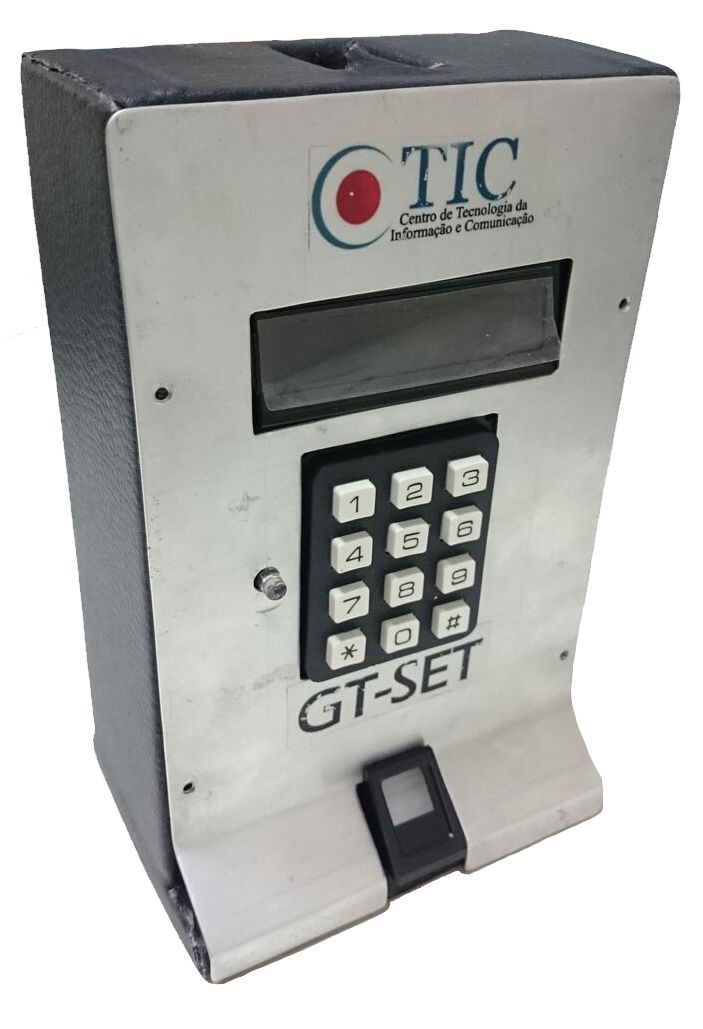
\includegraphics[scale=0.8]{figuras/cap4/setfinger_v1_1.jpg}\\
  Fonte: Elaborada pelo autor.
  \label{setfinger_v1_1}
  \end{center}
  \end{figure}
  
  
\begin{figure}[!t]
  \begin{center}
  \caption{Primeira versão de \textit{hardware} (SetFinger 1.0) - aparato eletrônico embutido em gabinete plástico}
  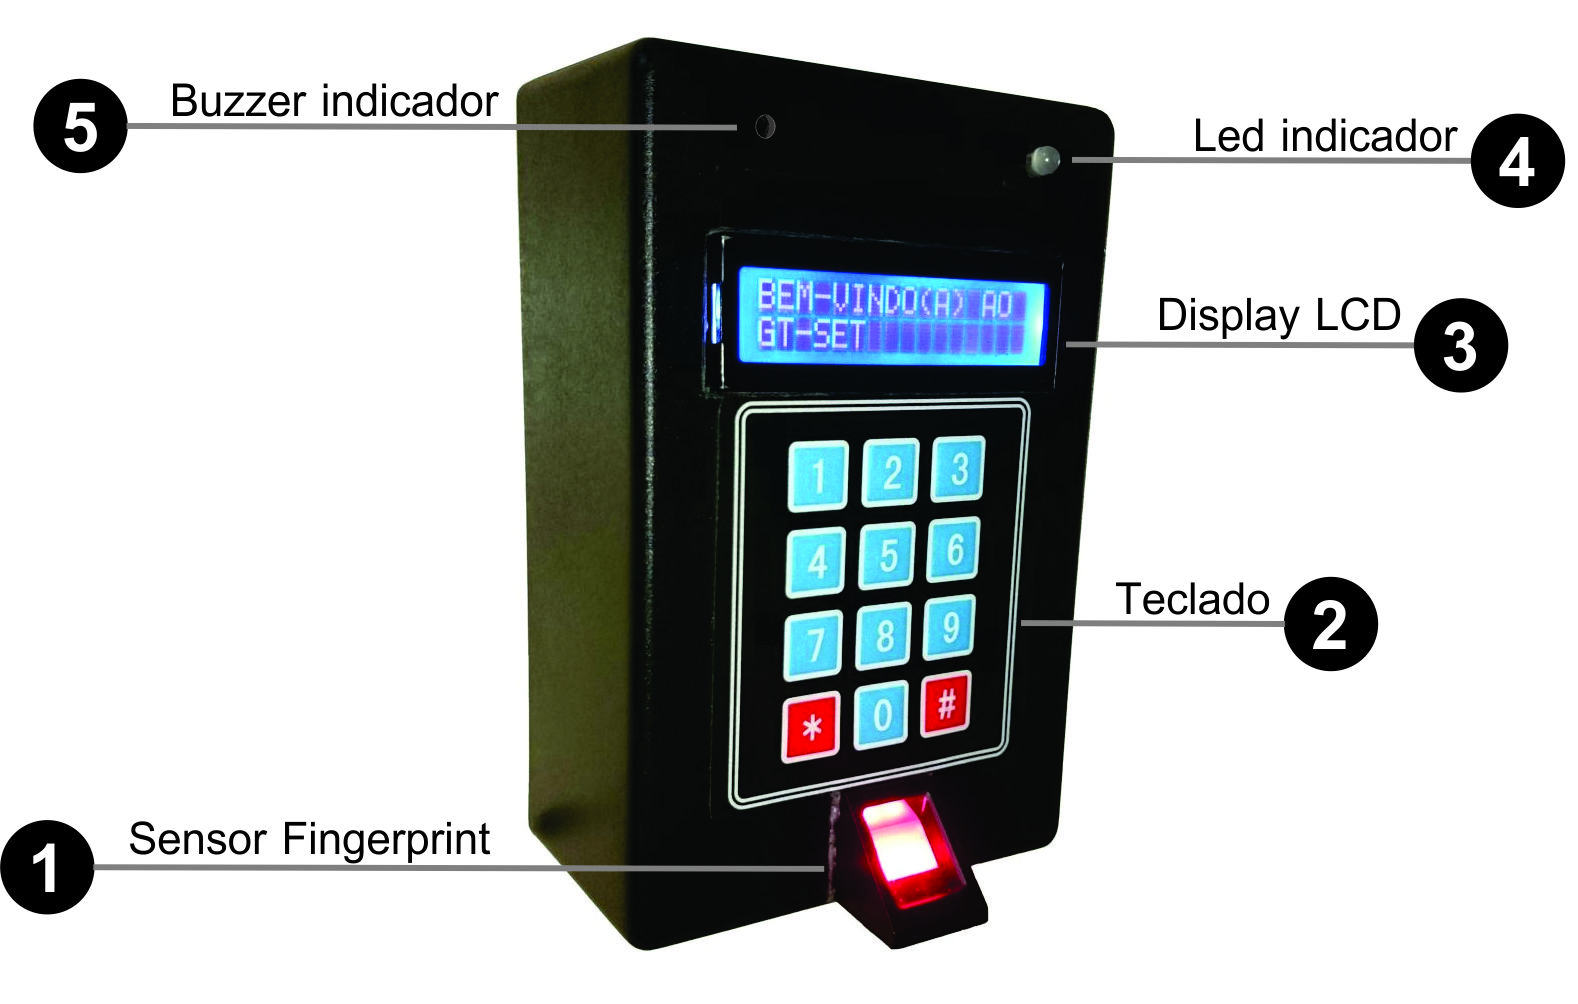
\includegraphics[scale=0.7]{figuras/cap4/setfinger_v1_2.jpg}\\
  Fonte: Elaborada pelo autor.
  \label{setfinger_v1_2}
  \end{center}
  \end{figure}


\begin{figure}[!t]
  \begin{center}
  \caption{Circuito de controle e proteção do fecho elétrico da versão de \textit{hardware} 1.0. Esse módulo de \textit{hardware} foi produzido somente na versão de aparelho Setfinger 1.0, nas demais versões o módulo de controle do fecho elétrico foi projetado na placa Setshield.}
  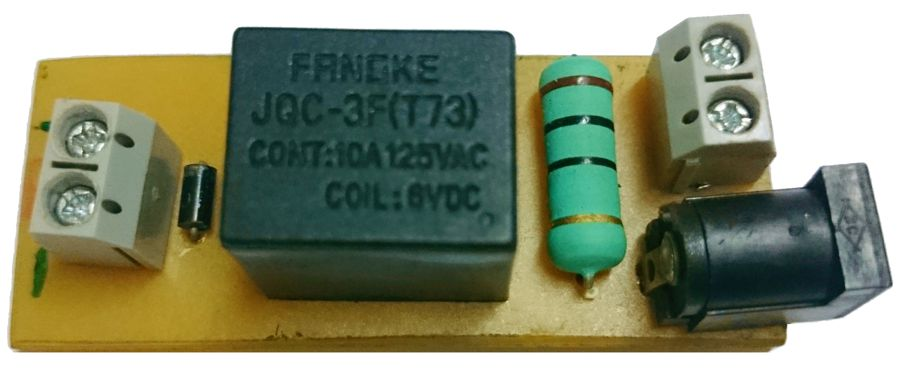
\includegraphics[scale=0.25]{figuras/cap4/circuito_fecho.jpg}\\
  Fonte: Elaborada pelo autor.
  \label{circuito_fecho}
  \end{center}
  \end{figure}
  

\begin{figure}[!t]
  \begin{center}
  \caption{Placa Setshield 1.0}
  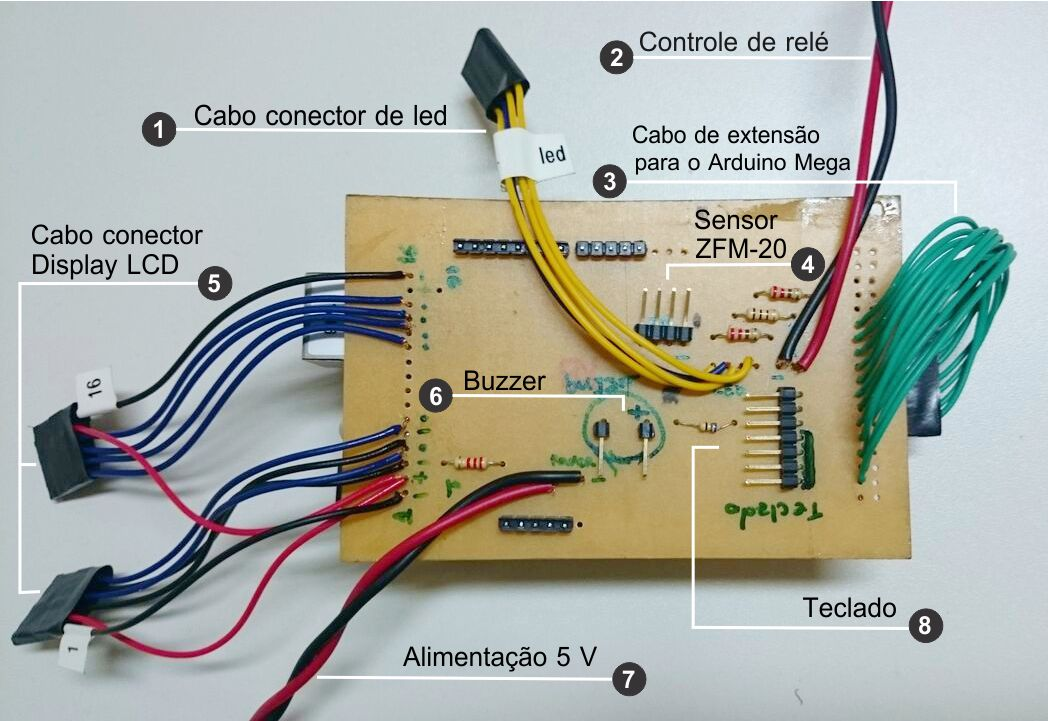
\includegraphics[scale=0.5]{figuras/cap4/setshield_v1.jpg}\\
  Fonte: Elaborada pelo autor.
  \label{setshield_v1}
  \end{center}
  \end{figure}




\chapter{Versão de \textit{hardware} Setfinger 2.0\label{hardware_2.0}}


Na segunda versão de \textit{hardware}, o aparelho Setfinger é dividido em dois módulos, por questões de segurança. Esses módulos são: um módulo interno à sala e um módulo externo,  (veja as Figuras~\ref{setfinger_v2} e ~\ref{setfinger_v2_p2}, respectivamente). Desta forma, o usuário só tem contato com o módulo externo, o qual é composto pelos seguintes componentes: teclado matricial, sensor fingerprint e Display LCD.  O módulo interno é composto pelo Arduino Mega, \textit{Ethernet Shield} e Setshield. As características gerais desse aparelho são apresentadas a seguir:


\begin{itemize}

\item Alimentação

O Arduino e os componentes conectados à ele, são alimentados pela mesma fonte utilizada para acionar a fechadura eletrônica, uma fonte chaveada de $12$ V/$5$ A. Para isso, foi utilizado um regulador de 5V, modelo 708S05, a fim de eliminar a fonte de $5$ V utilizada na versão 1.0 para alimentar o Arduino. 

\item Fechadura eletrônica

O aparelho Setfinger é integrado a um fecho eletromagnético de $12$ V/200 mA. 


O fecho é conectado diretamente ao módulo de \textit{hardware} interno, que contém um relé acoplado à placa Setshield. Desta forma, o fecho é acionado para liberar a abertura da porta, quando o relé é acionado com um sinal elétrico de $5$ V. 

\item Setshield

O setshield, mostrado na Figura~\ref{setshield_v2}, é a PCB que conecta ao Arduino os seguintes dispositivos: display LCD, teclado matricial, sensor fingerprint, buzzer, led e relé. Todas as conexões entre esses dispositivos e placa Setshield, são feitas por meio de cabos conectados em barras de pinos soldados à PCB. 

\item Conexão com o Arduino Mega

A placa Setshield foi conectada aos pinos do Arduino Mega, não alcançados por barra de pinos, através de um cabo de extensão, assim como na versão 1.0. No entanto, diferente da versão 1.0, o cabo não foi soldado à placa Setshield. As extremidades do cabo foram conectadas por meio de encaixe.


\end{itemize}



\begin{figure}[!ht]
  \begin{center}
  \caption{Segunda versão de \textit{hardware} (Setfinger 2.0) - módulo de interface com o usuário, composto por um display LCD, um leitor de impressões digitais e um teclado matricial do tipo membrana, embutidos em um gabinete plástico. Este módulo deve ser instalado do lado externo do ambiente a ser controlado e próximo a porta}
  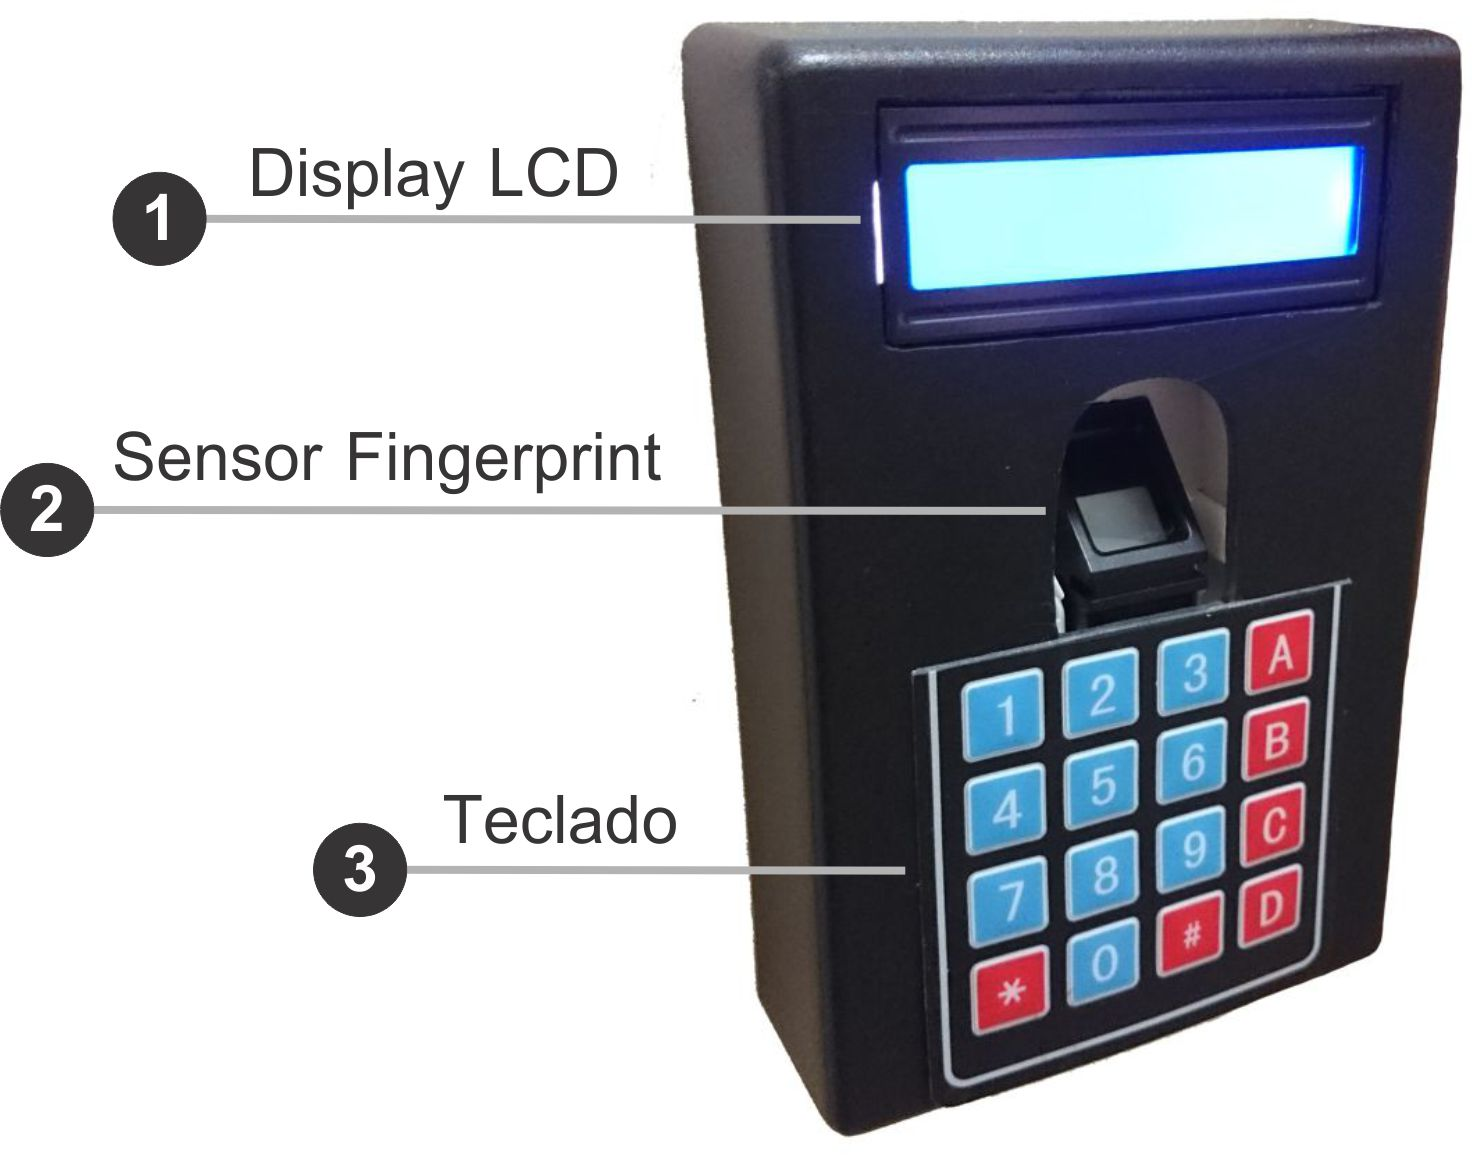
\includegraphics[scale=0.2]{figuras/cap4/setfinger_v2.jpg}\\
  Fonte: Elaborada pelo autor.
  \label{setfinger_v2}
  \end{center}
  \end{figure}

\begin{figure}[!ht]
  \begin{center}
  \caption{Segunda versão de \textit{hardware} (SetFinger 2.0) - módulo de \textit{hardware} interno composto por um Arduino Mega 2560, um ethernet shield W5100 e um Setshield 2.0. Esse módulo deve ser instalado fora do alcance dos usuários, preferencialmente no interior da sala a ser controlada.}
  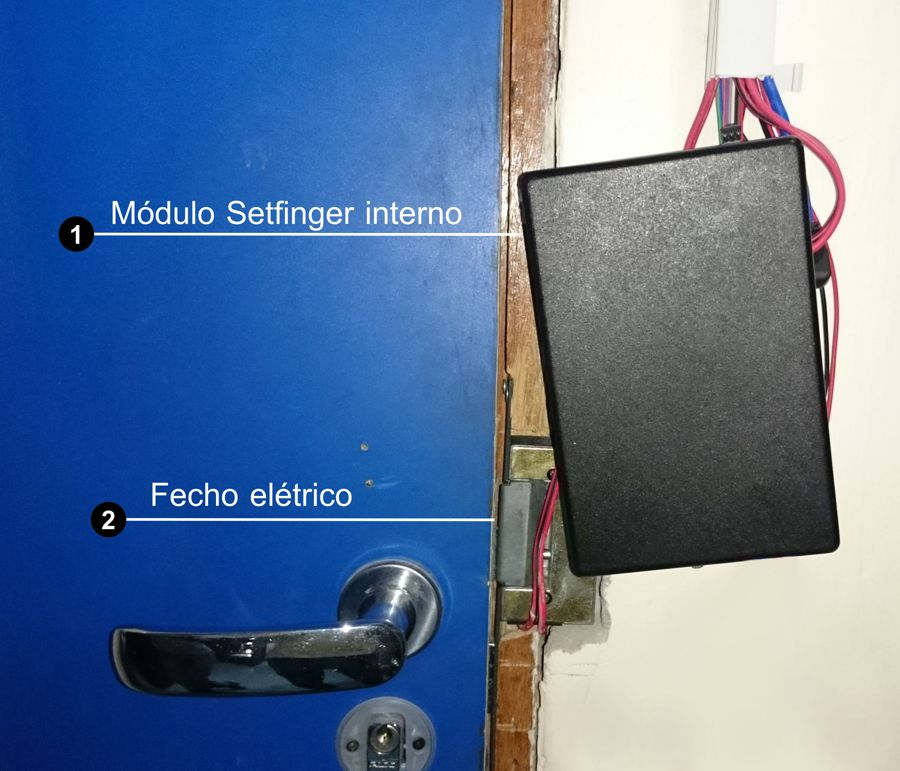
\includegraphics[scale=0.5]{figuras/cap4/setfinger_v2_p2.jpg}\\
  Fonte: Elaborada pelo autor.
  \label{setfinger_v2_p2}
  \end{center}
  \end{figure}
  

\begin{figure}[!ht]
  \begin{center}
  \caption{Placa Setshield 2.0.}
  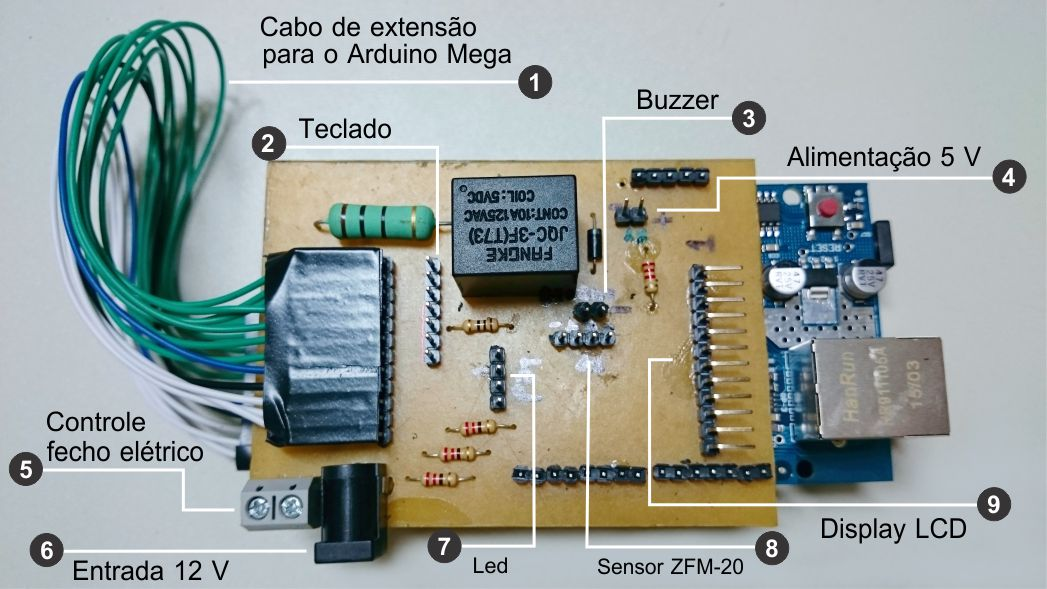
\includegraphics[scale=0.55]{figuras/cap4/setshield_v2.jpg}\\
  Fonte: Elaborada pelo autor.
  \label{setshield_v2}
  \end{center}
  \end{figure}


\chapter{Esquemático da placa Setshield \label{schematic_setshield}}

Esquemático da placa Setshield projetada no \textit{softwate} CadSoft Eagle 7.5.0.
  \begin{center}
  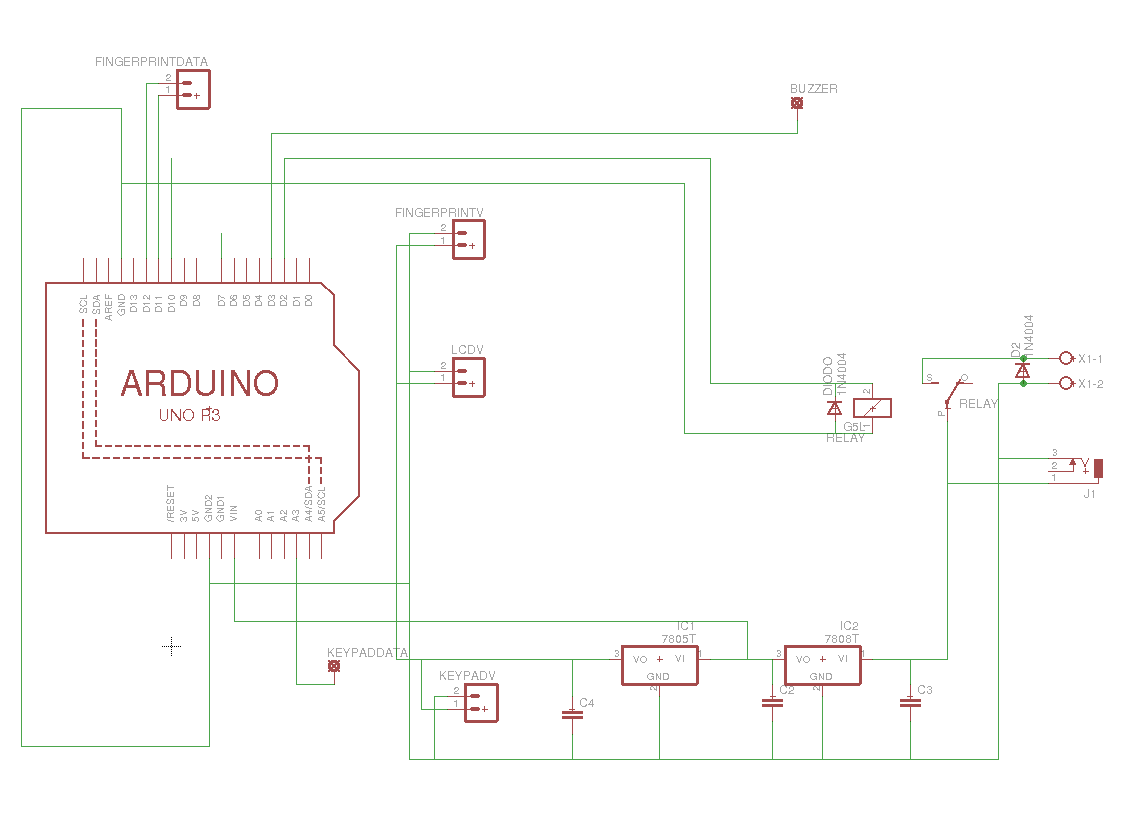
\includegraphics[scale=0.55]{figuras/anexos_e_apendices/schematic_setshield.png}\\
  Fonte: Elaborada pelo autor.
  \end{center}


\chapter{Design da placa Setshield \label{board_setshield}}

Design da placa Setshield projetada no \textit{softwate} CadSoft Eagle 7.5.0.

  \begin{center}
  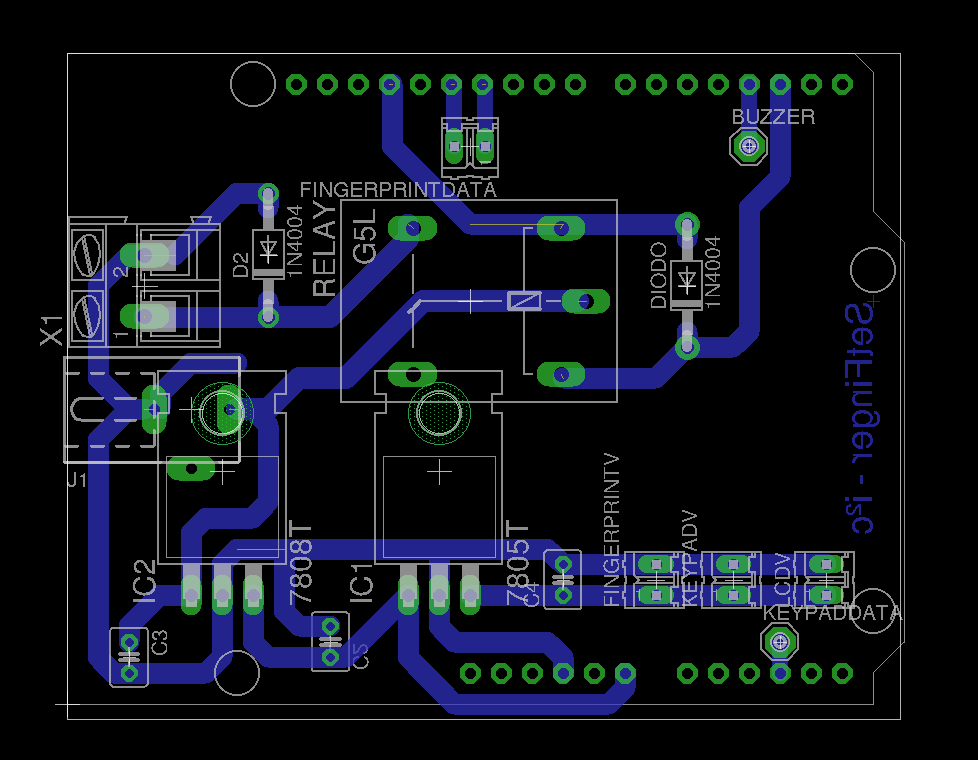
\includegraphics[scale=0.55]{figuras/anexos_e_apendices/board_setshield.png}\\
  Fonte: Elaborada pelo autor.
  \end{center}
  
\newpage